\section{Durchführung}
\subsection{Aufbau und Justage}
Der Aufbau besteht aus 

\begin{itemize}
  \item einem Permanentmagneten,
    \item einem PS2-Controller zur Regelung der Magnettemperatur und des Magnetfeldgradienten,
      \item dem Mainframe an dem die Pulssequenzen eingestellt werden und
        \item einem digitalen Oszilloskop.
\end{itemize}

Zunächst wird mit dem PS2 Controller eingestellt, dass die aktuelle Magnettemperatur gehalten wird. Dies ist wichtig, da sich sonst das Megnetfeld bei Temperaturschwankungen ändern kann. \\ \\
Für eine erste Justage wird nun die Pickup-Probe in den Magneten eingesetzt. Diese besteht aus einer einfachen Spule. An dem Mainframe wird als Puls ein Rechteckpuls (Puls A) mit Pulslänge $A_{len}=2,5\mu$s eingestellt. Die Periode (nach welcher Zeit die Pulssequenz sich wiederholt) wird auf $100$ms gestellt. Es muss immer darauf geachtet werden, dass die Periode deutlich größer als die Pulslänge ist. Auf dem Oszilloskop kann nun eine zum Strom der Spule proportionale Spannung beobachtet werden (siehe Abbildung \ref{fig:pickup}). Das Signal hat bereits die erwünschte Form und es sind keine Einstellungen am Magneten notwendig.\\ \\
Nun wird die eigentliche Probe mit Mineralöl in den Magneten eingesetzt. Auf dem Oszilloskop kann nun nach einem $\pi/2$ Puls das FID Signal beobachtet werden. Die Dauer für einen $\pi/2$-Puls wird ermittelt indem die Amplitude des Antwortsignals maximiert wird. Die so ermittelte Pulslänge liegt bei $2,46 \mu$s. Die Frequenz des RF-Pulses und der Magnetfeldgradient werden so eingestellt, dass die Amplitude und die Zerfallszeit des FID Signals maximal werden und keine Nachschwingungen zu erkennen sind. Die ermittelte Resonanzfrequenz liegt bei $21,16272$MHz. Das FID Signal ist in Abbildung \ref{fig:FID} zu sehen. \\ \\
Für eine genauere Bestimmung der Zeit für einen $\pi/2$-Puls wird die Zeit für einen $\pi$-Puls bestimmt indem das Antwortsignal minimiert wird. Die ermittelte Zeit für einen $\pi$-Puls ist $4,92\mu$s, welche genau zu unserer Zeit für den $\pi/2$-Puls passt.

\subsection{Rabi-Oszillationen}
Für Puls A und Pulslängen zwischen $0,5\mu$s und $12\mu$s wird die Magnetisierung in der x-y-Ebene gemessen. Gemessen wird dabei sowohl die Amplitude in der Ebene (Envelope Signal) als auch in einer Raumrichtung der Ebene (In-Phase Signal). Erwartet wird ein oszillierendes Signal in Abhängigkeit der Pulslänge. 

\subsection{Longitudinale Relaxationszeit}
Die Longitudinale Relaxationszeit wird mit zwei verschiedenen Methoden gemessen. \\ \\
Bei der Sättigungs-Zurückgewinnung wird die Probe zunächst einem $\pi/2$-Puls ausgesetzt und anschließend nach einer Wartezeit $\tau$ die Magnetiserung in z-Richtung gemessen (wieder durch einen $\pi/2$-Puls). Durch die Variation von $\tau$ lässt sich die longitudinale Relaxationszeit ermitteln. \\ \\
Bei der Polarisations-Zurückgewinnung unterscheidet sich das Prozedere nur dahingehend, dass die Probe zu Beginn einem $\pi$-Puls ausgesetzt wird. Dadurch wird die Magnetisierung in die negative z-Richtung gedreht. Wieder wird die Amplitude für verschiedene $\tau$ aufgenommen.

\subsection{Homogene Transversale Relaxationszeit}
Die homogene transversale Relaxationszeit wird mit den drei vorgestellten Pulssequenzen ermittelt. Bei der Hahn-Spinecho-Sequenz wird dazu manuell für verschiedene Wartezeiten $\tau$ das Antwortsignal aufgenommen. Bei der Carr-Purcell und der Meiboom-Gill-Sequenz reicht eine Pulssequenz mit $N=20$ Perioden.\\ \\
Um die Carr-Purcell und die Meiboom-Gill-Sequenz vergleichen zu können wird noch die Änderung der Signale bei variierendem Magnetfeldgradienten untersucht.

\begin{figure}[h]
  \centering
  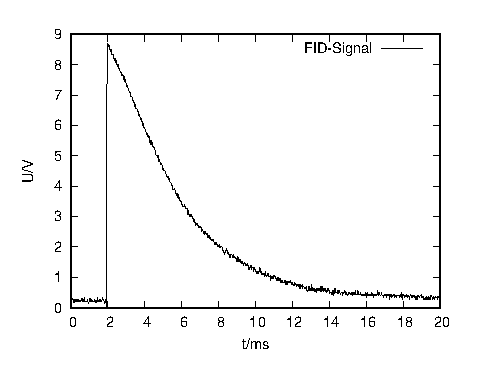
\includegraphics[width=0.75\linewidth]{data/p402_443_data/FID_1/FID_1.eps}
  \caption{FID Signal}
  \label{fig:FID}
\end{figure}
